\documentclass[11pt]{article}
\usepackage{ctex, amsmath, amssymb, graphicx, float, xcolor, bbm}
\usepackage[a4paper, margin=1in]{geometry}
\usepackage{caption, subcaption}
\usepackage{hyperref}
\hypersetup{colorlinks=true, urlcolor=blue, linkcolor=black}

\title{SimCLR-Based Self-Supervised Learning on CIFAR-10: Experimental Report}
\author{刘行 PB22000150}
\date{\today}

\begin{document}

\maketitle

\section{\textbf{引言}}
随着深度学习的发展, \textbf{自监督学习 (Self-Supervised Learning, SSL)}逐渐成为替代有监督学习标注成本的一种有效手段. SimCLR 是 Google 提出的对比式自监督框架, 其核心思想是通过最大化正样本对之间的一致性以学习判别特征表示.

本报告旨在实现并分析 SimCLR 框架在 CIFAR-10 子集上的表现, 通过比较不同的数据增强策略和投影头结构, 评估其对自监督训练与下游分类任务的影响.

\section{\textbf{数学原理与模型结构}}

\subsection{\textbf{对比学习损失 NT-Xent}}
设一个 batch 中含有 $N$ 张图像, 每张图像经过两种不同的数据增强策略生成两个视图, 共 $2N$ 个样本. 对于每对来自同一原图像的视图 $(\mathbf{z}_i, \mathbf{z}_j)$, 定义它们为正样本对, 其余为负样本.

相似度使用归一化余弦相似度定义:
\begin{equation}
\text{sim}(\mathbf{z}_i, \mathbf{z}_j) = \frac{\mathbf{z}_i^\top \mathbf{z}_j}{|\mathbf{z}_i||\mathbf{z}_j|}
\end{equation}

NT-Xent (Normalized Temperature-scaled Cross Entropy) 损失为:
\begin{equation*}
\mathcal{L}_{i,j} = -\log \frac{\exp(\text{sim}(\mathbf{z}*i, \mathbf{z}*j)/\tau)}{\sum_{k=1}^{2N} \mathbbm{1}_{[k \ne i]} \exp(\text{sim}(\mathbf{z}_i, \mathbf{z}_k)/\tau)}
\end{equation*}

总损失为所有正样本对的平均:
\begin{equation*}
\mathcal{L} = \frac{1}{2N} \sum_{i=1}^{2N} \mathcal{L}_{i, j(i)}
\end{equation*}
其中, $\tau$ 为温度系数, 控制分布的平滑程度, $j(i)$ 通过 $j(i) = (i + N) \% 2N$ 得到.

\subsection{\textbf{模型结构}}
SimCLR 模型结构包括:
\begin{itemize}
\item \textbf{基础编码器} (Base Encoder): 使用 ResNet18 作为特征提取器, 去除最大池化与分类层.
\item \textbf{投影头} (Projection Head): 一个将高维表征映射到对比空间的小型神经网络, 其结构对性能有显著影响.
\end{itemize}

\section{\textbf{代码结构与实现思路}}

\subsection{数据加载与增强}
使用 torchvision 加载 CIFAR-10, 选取全部数据作为训练集. 通过 \texttt{SimCLRDataset} 生成正样本对, 支持 \texttt{basic, color, gray, strong} 四种增强策略.

\subsection{SimCLR 模型实现}
\begin{itemize}
\item \texttt{SimCLR}: 包含 encoder 和投影头, 支持多种 head 类型: \texttt{mlp\_bn, mlp\_no\_bn, linear, none}.
\item \texttt{LinearClassifier}: 用于冻结 encoder 后进行线性评估.
\end{itemize}

\subsection{训练流程}
\begin{enumerate}
\item 对比学习阶段: 训练 SimCLR 模型最小化 NT-Xent 损失;
\item 线性评估阶段: 冻结 encoder, 仅训练一个线性分类器;
\item 实验日志 (\texttt{result/output.txt}) 和模型 (\texttt{checkpoints/xx\_xx.pth}) 保存在统一路径下, 输出写入统一文件用于绘图.
\item 单独使用 \texttt{result\_plot.py} 脚本加载格式化的输出数据并绘制训练损失和线性评估准确率.
\end{enumerate}

\section{\textbf{实验设置}}

\subsection{训练配置}
\begin{itemize}
\item Batch size: 256
\item Epochs: 100 (pretrain), 50 (eval)
\item Optimizer: Adam
\item Temperature: 0.1
\item Projection dim: 128
\end{itemize}

\subsection{实验维度}
本报告分析两个关键变量: 
\begin{itemize}
\item \textbf{增强策略} (tag 1--4): basic, color, gray, strong
\item \textbf{投影头结构} (tag 5--8): mlp\_bn, mlp\_no\_bn, linear, none
\end{itemize}

\section{\textbf{实验结果}}

\subsection{预训练损失 (Pretraining Loss)}
如图 1 和图 2 所示, 在增强策略和投影头结构维度上, SimCLR 的训练损失均随 epoch 稳定下降.

\begin{figure}[htbp]
	\centering
	\begin{subfigure}[htbp]{0.45\textwidth}
		\centering
		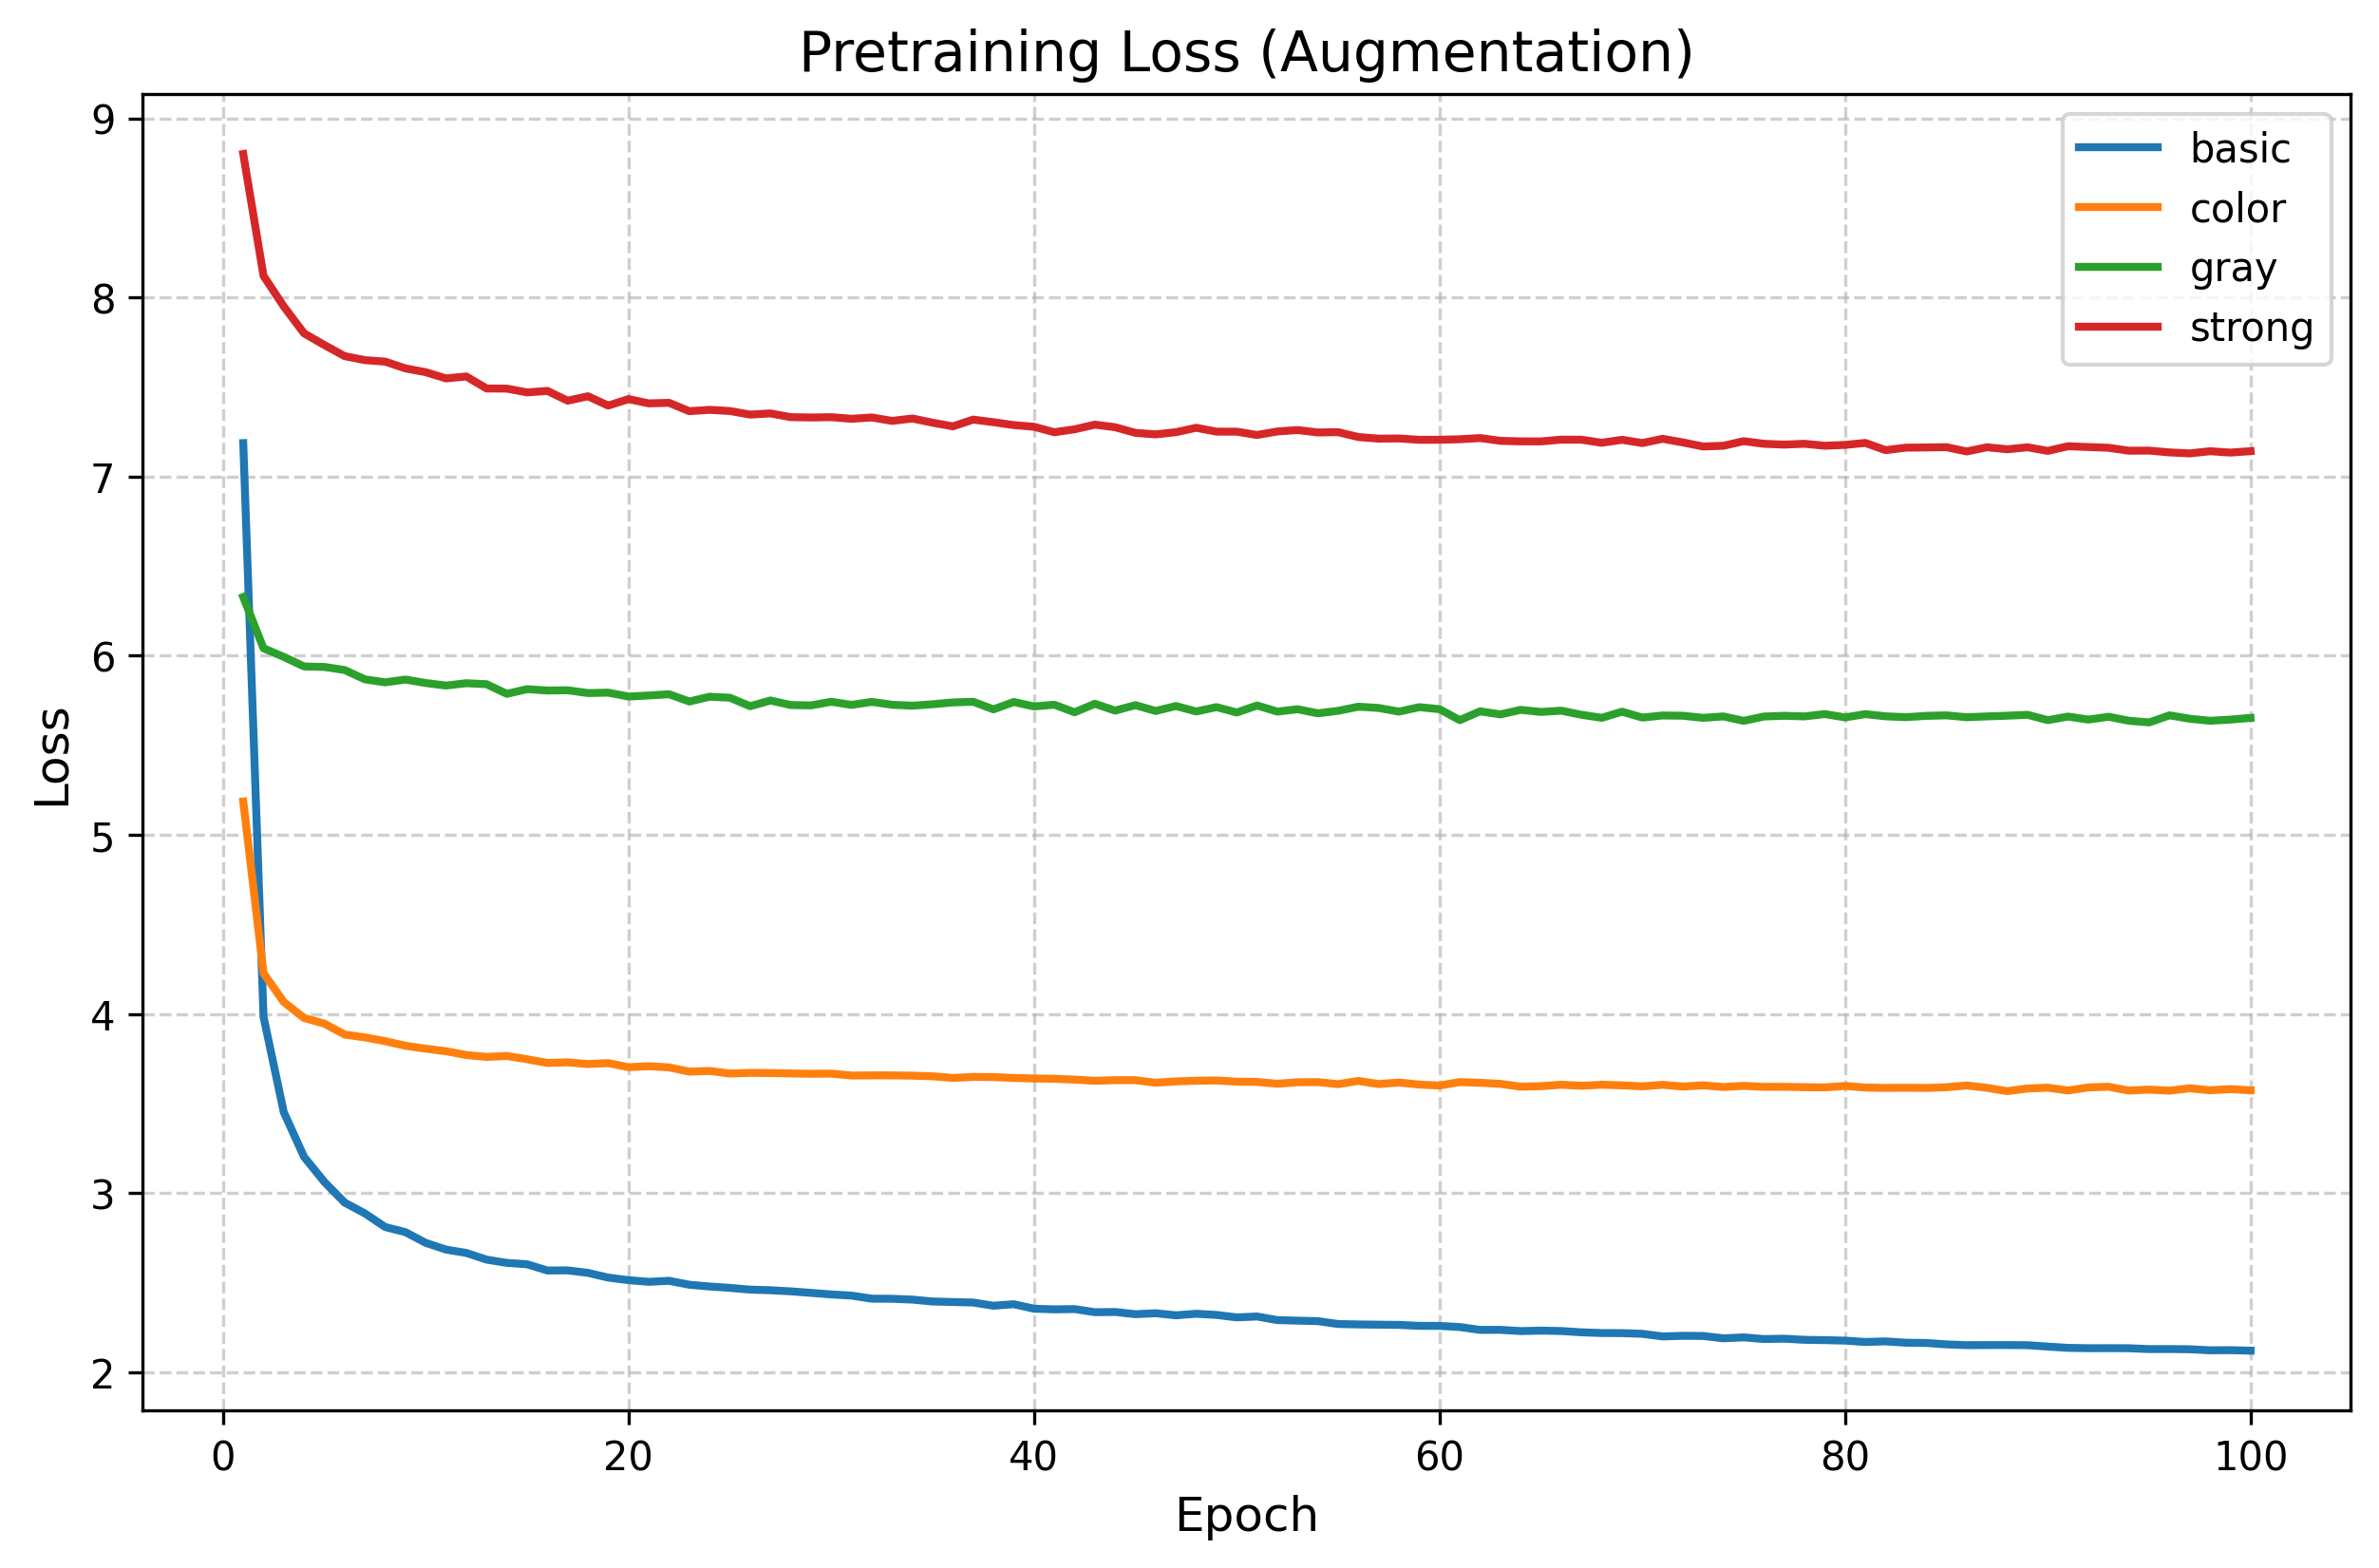
\includegraphics[width=\textwidth]{figure/pretrain_loss_augment.png}
		\caption{不同增强策略下的预训练损失}
	\end{subfigure}
	\hfill
	\begin{subfigure}[htbp]{0.45\textwidth}
		\centering
		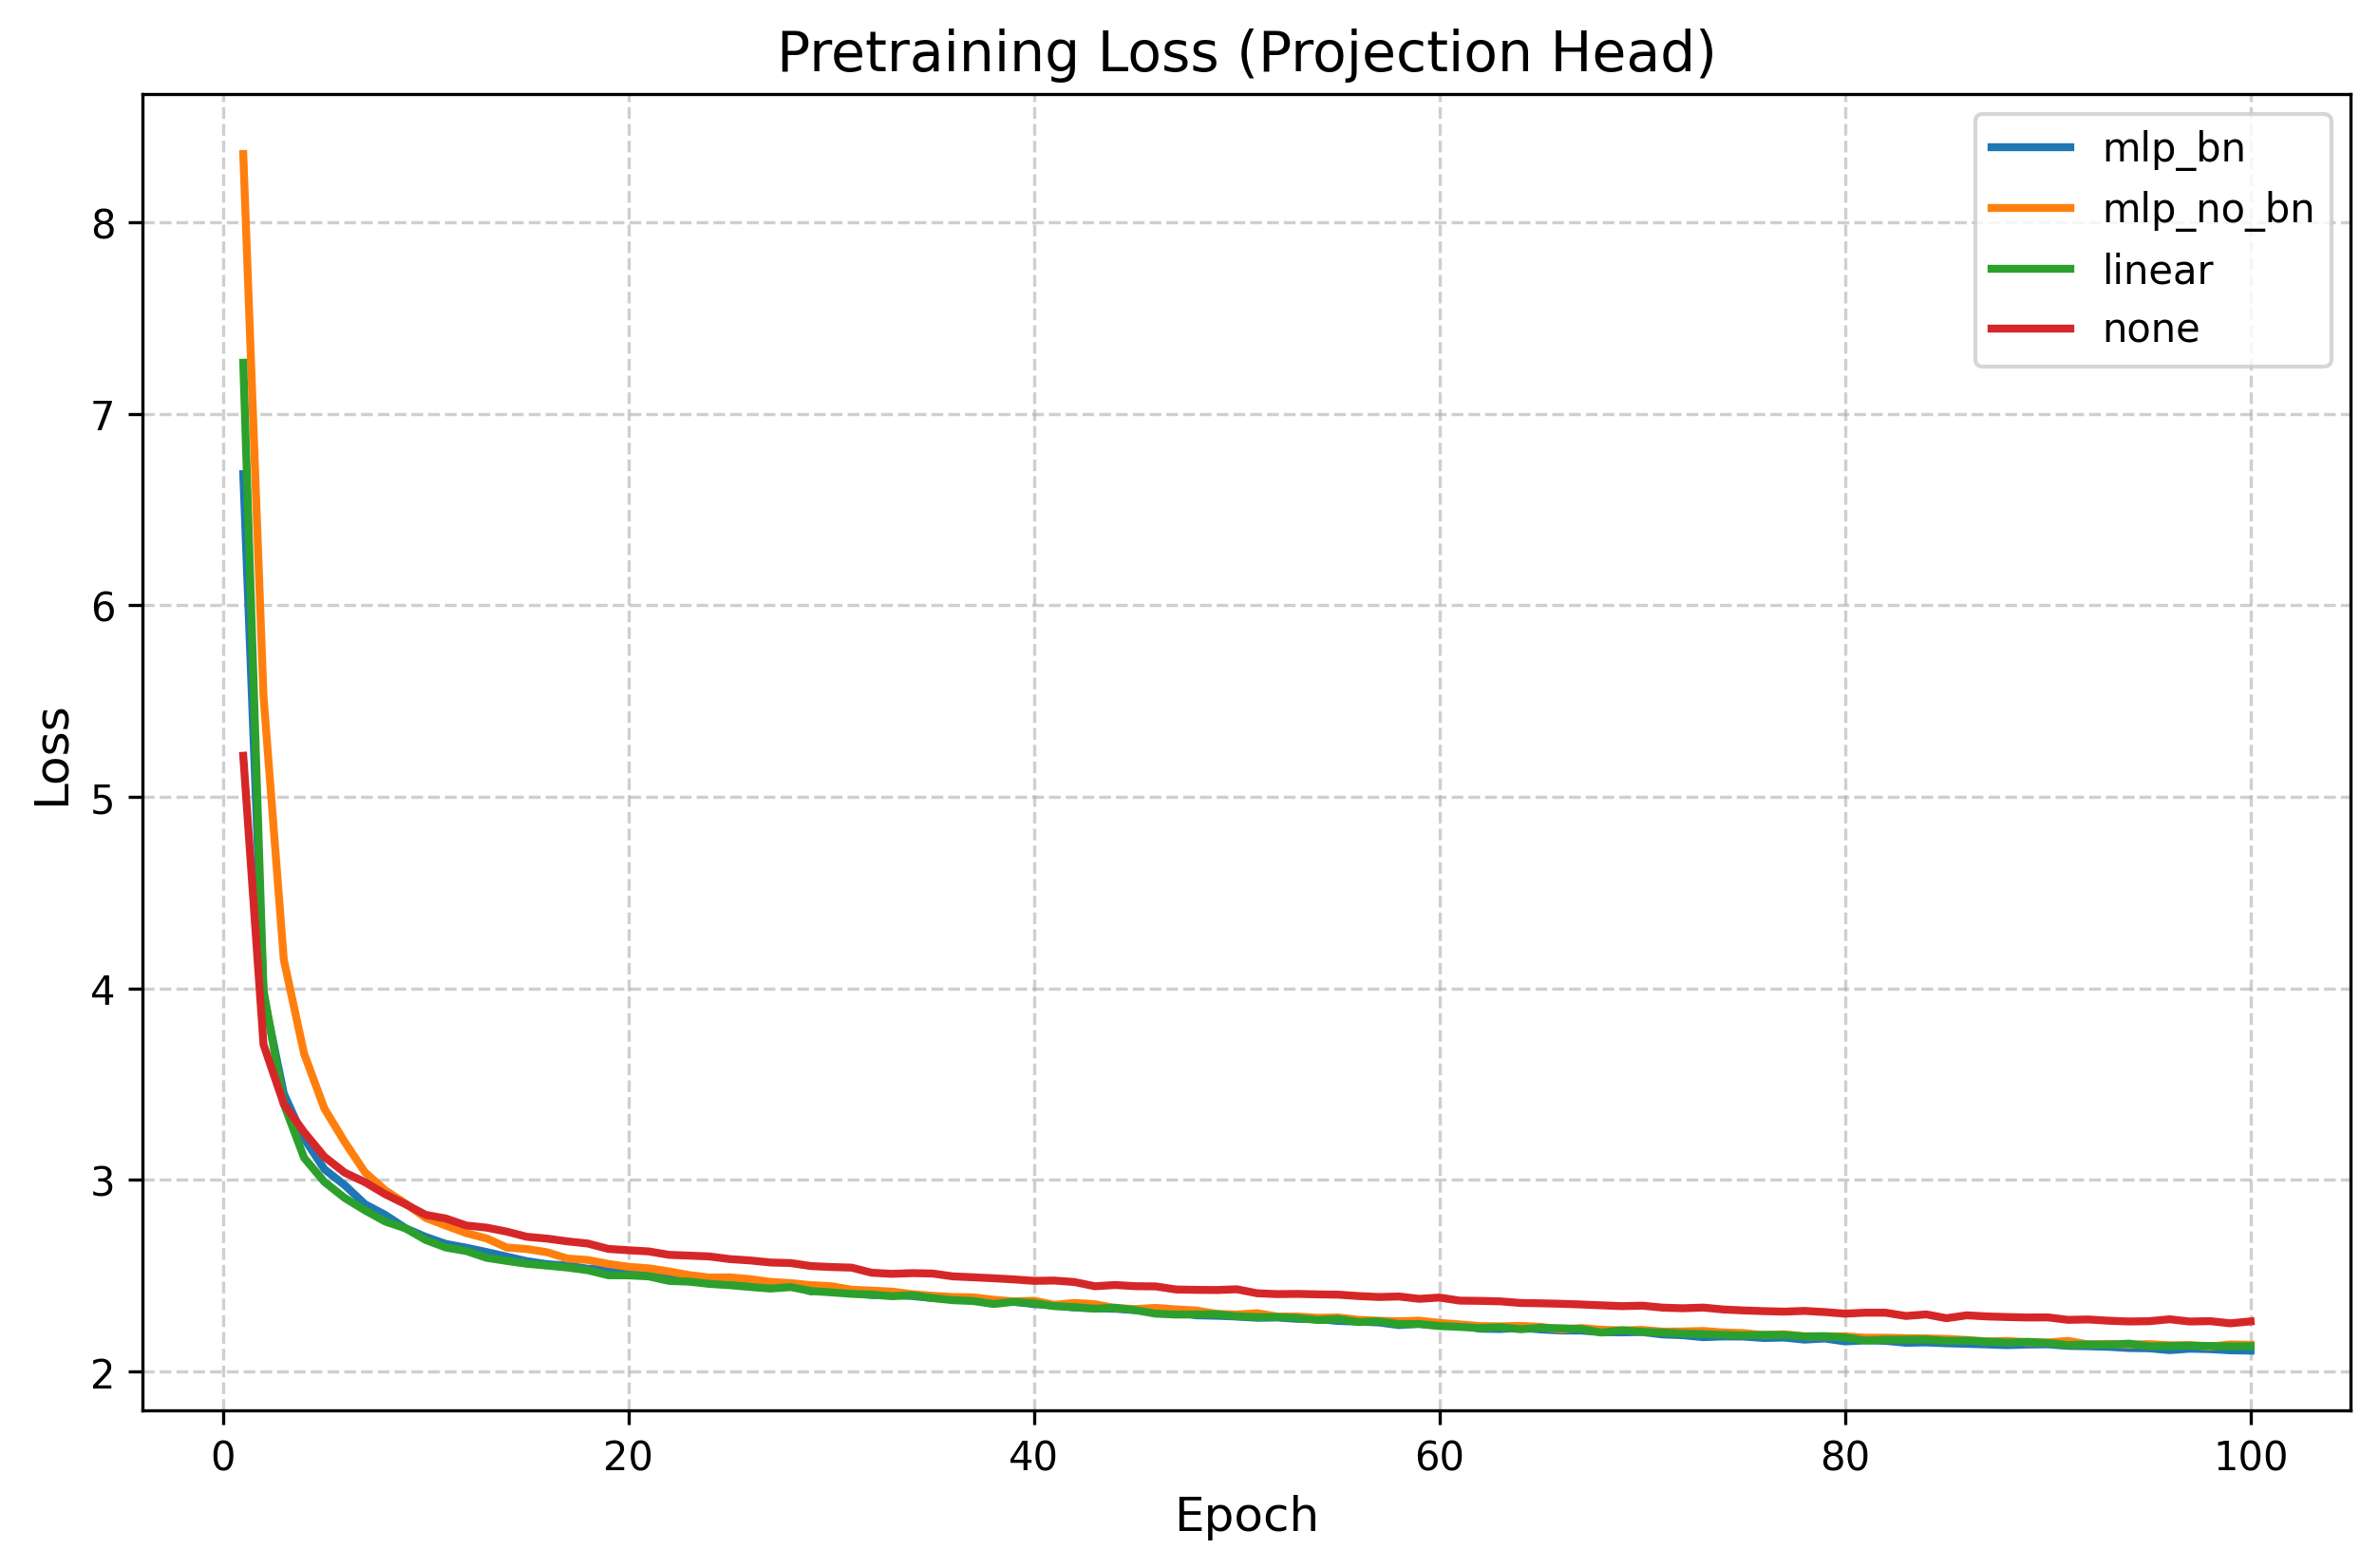
\includegraphics[width=\textwidth]{figure/pretrain_loss_head.png}
		\caption{不同投影头结构下的预训练损失}
	\end{subfigure}
	\caption{预训练损失比较}
\end{figure}

\subsection{评估准确率 (Linear Evaluation Accuracy)}
在固定 encoder 后训练线性分类器, 评估在测试集上的表现, 如图 3 和图 4 所示: 

\begin{figure}[htbp]
	\centering
	\begin{subfigure}[htbp]{0.45\textwidth}
		\centering
		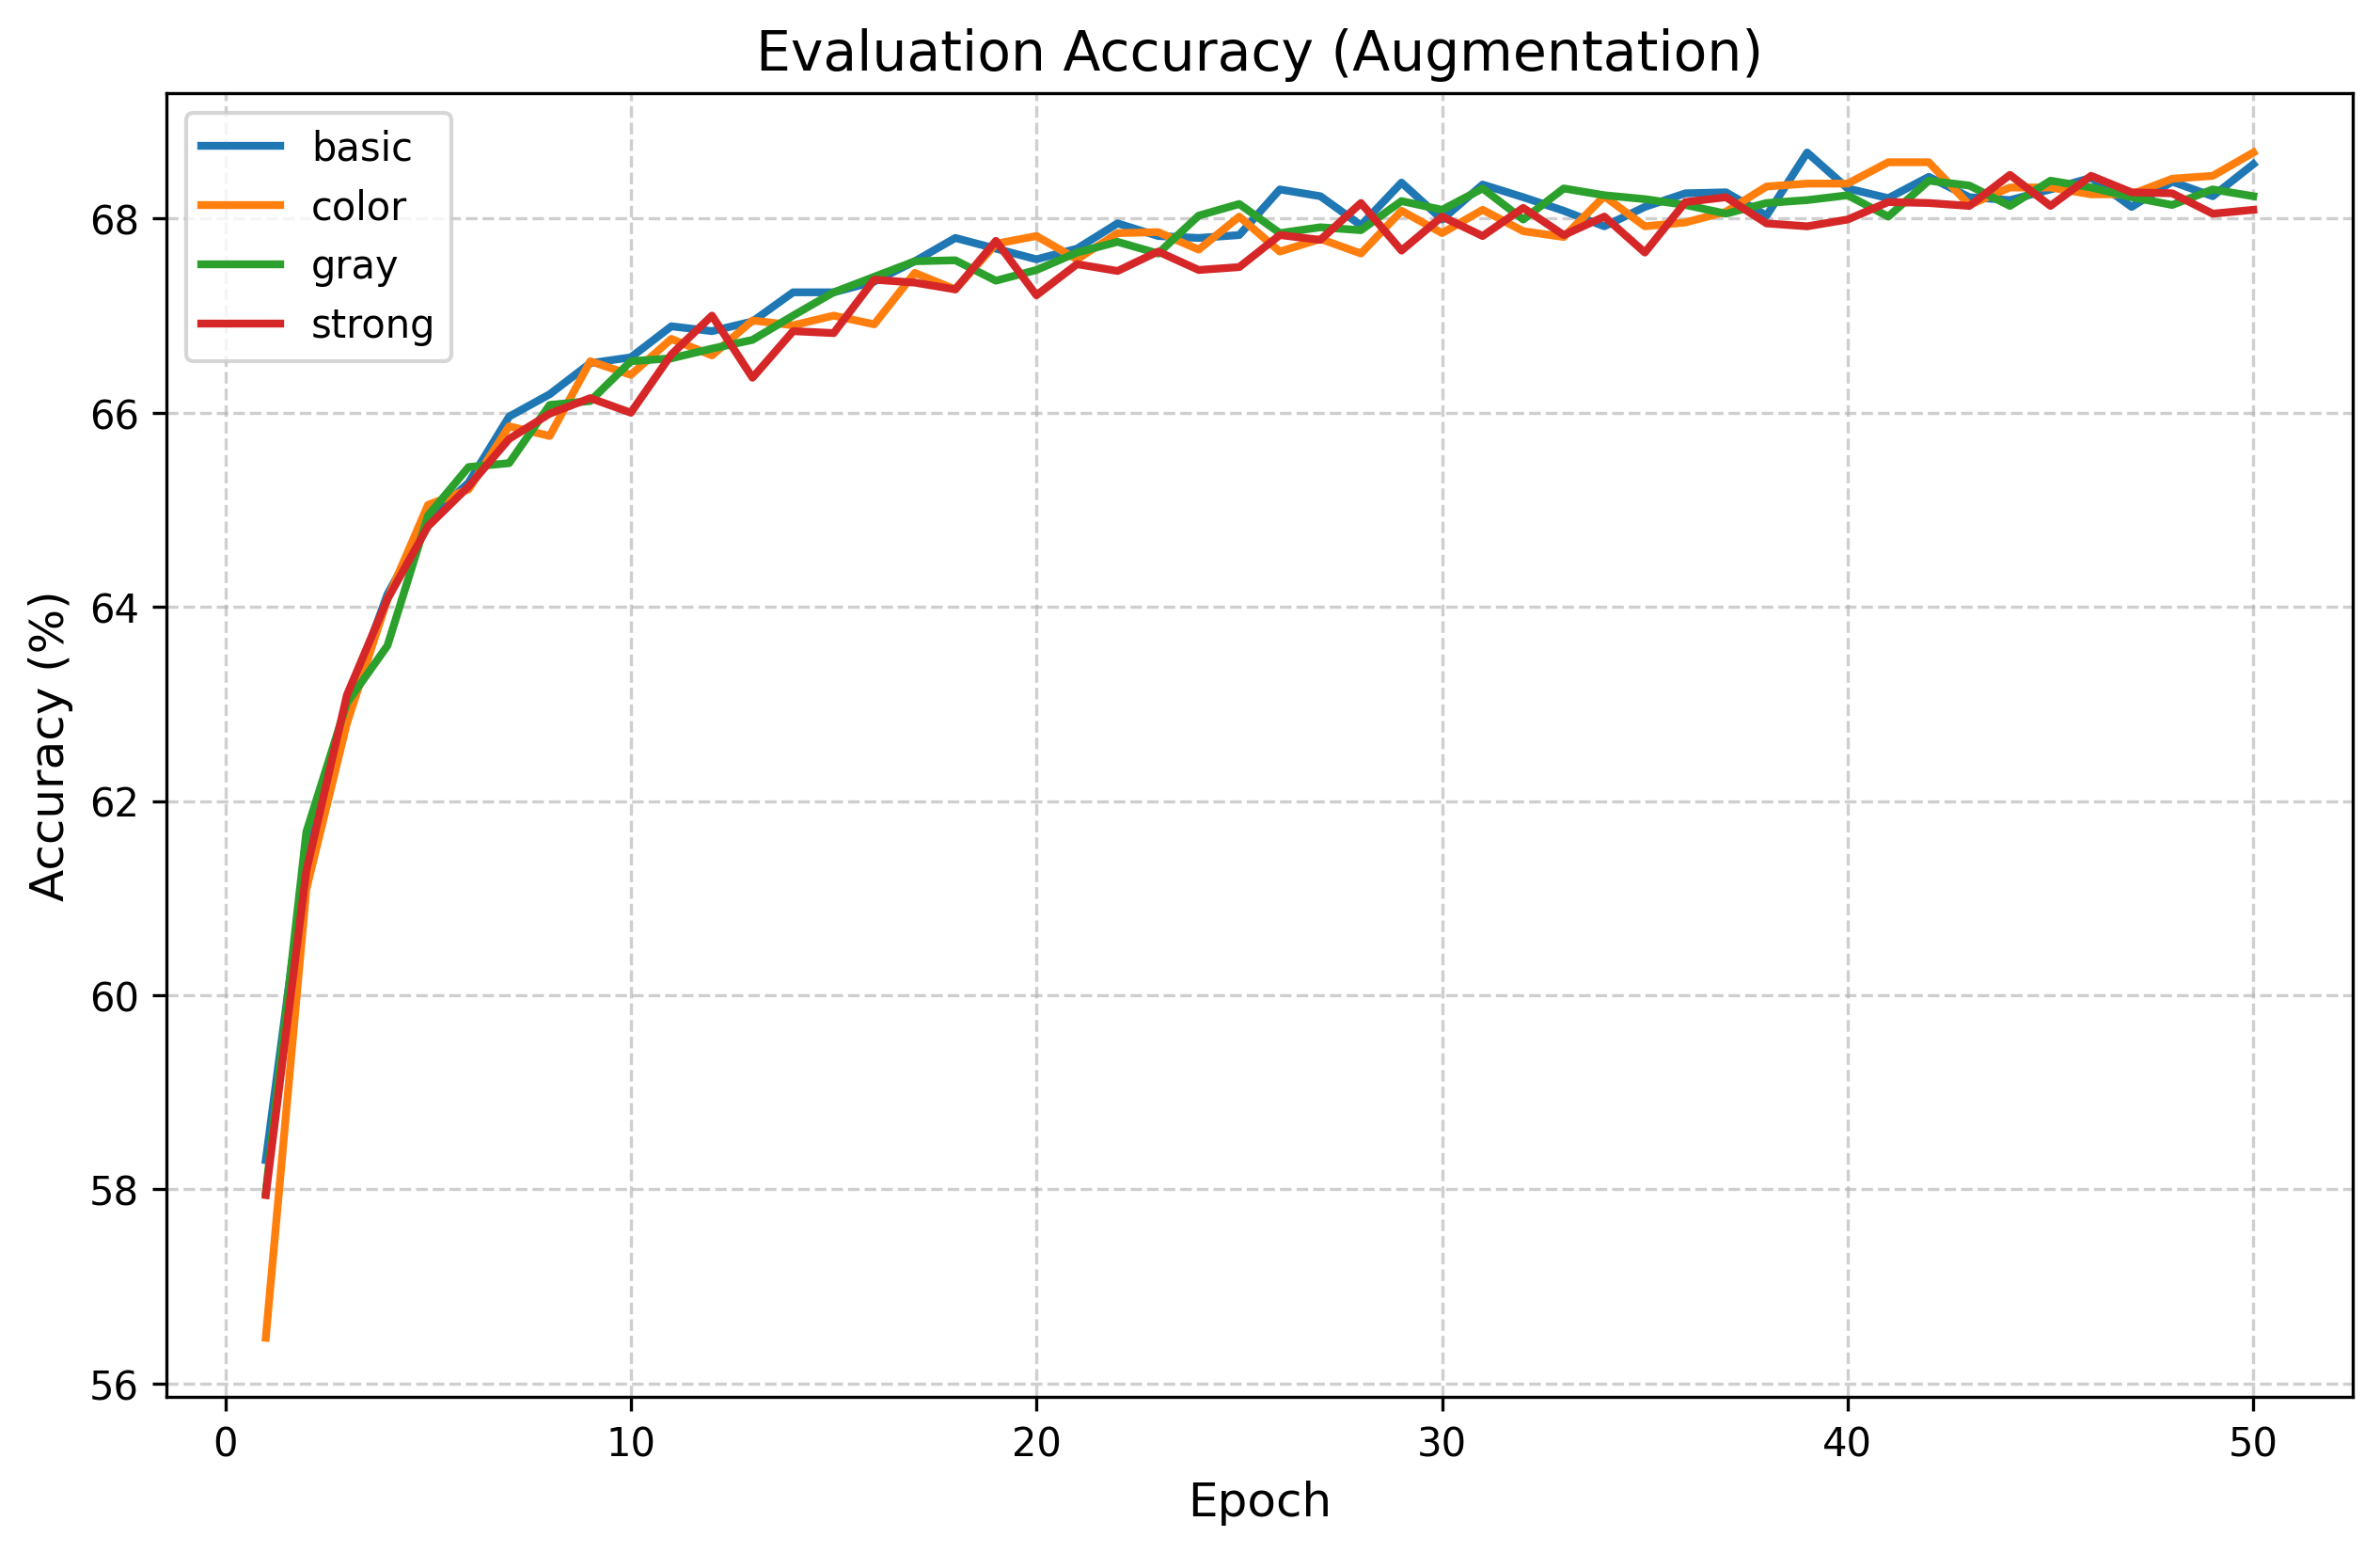
\includegraphics[width=\textwidth]{figure/eval_acc_augment.png}
		\caption{不同增强策略下的线性评估准确率}
	\end{subfigure}
	\hfill
	\begin{subfigure}[htbp]{0.45\textwidth}
		\centering
		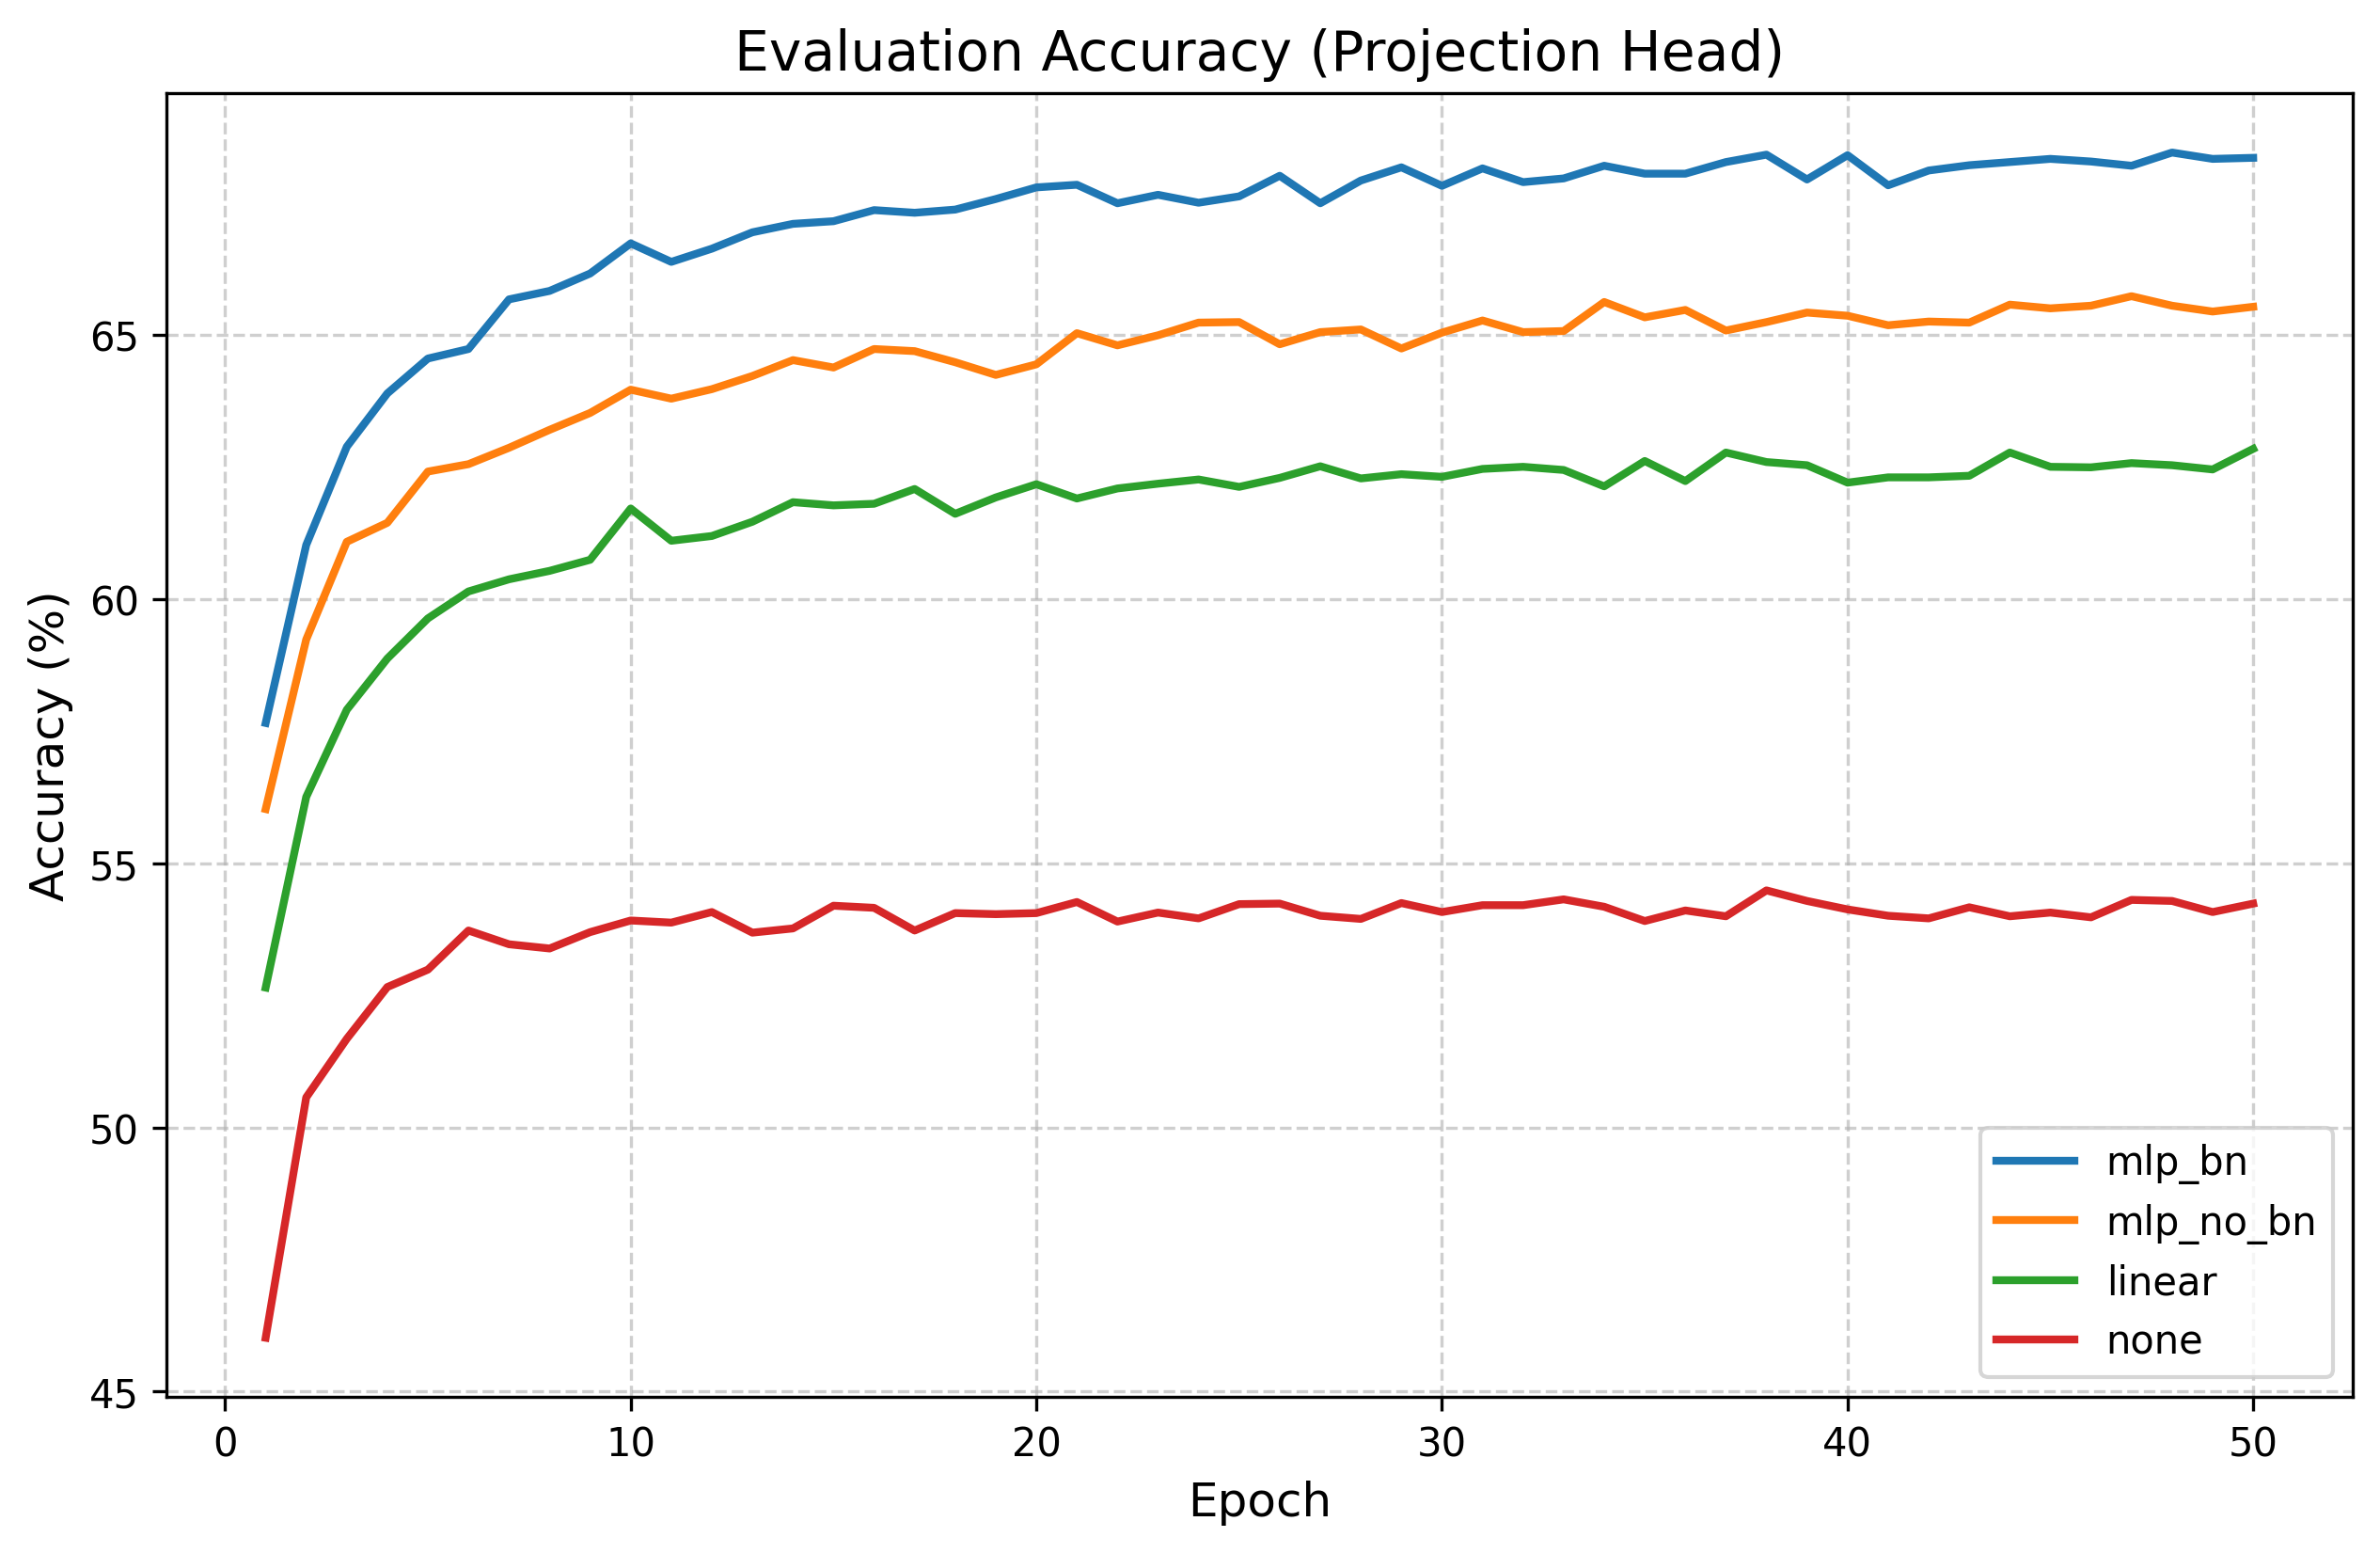
\includegraphics[width=\textwidth]{figure/eval_acc_head.png}
		\caption{不同投影头结构下的线性评估准确率}
	\end{subfigure}
	\caption{线性评估准确率比较}
\end{figure}

\section{\textbf{实验分析}}

\subsection{增强策略影响}
\begin{itemize}
\item 使用 \texttt{color} 和 \texttt{gray} 增强并没有显著提升表示的判别性, 准确率与 \texttt{basic} 相差无几.
\item \texttt{strong} 增强未必最优, 可能对小数据集造成过拟合.
\end{itemize}

\subsection{投影头结构影响}
\begin{itemize}
\item 原始设计 (\texttt{mlp\_bn}) 表现最佳, 说明非线性和 BatchNorm 有利于对比学习空间.
\item 单层线性 (\texttt{linear}) 与无投影 (\texttt{none}) 准确率下降明显.
\end{itemize}

\section{\textbf{结论与展望}}
本实验验证了 SimCLR 在小规模 CIFAR-10 数据子集上的有效性, 增强策略与投影头结构均对最终表示性能有显著影响.

未来工作可扩展至:
\begin{itemize}
\item 不同温度参数, batch size 的系统性对比;
\item encoder 结构变体 (如 ResNet34, ViT);
\item TSNE 或类间距离分析进一步理解表示空间结构.
\end{itemize}

\end{document}
